\hypertarget{graphics_8c}{
\section{Referencia del Archivo graphics.c}
\label{graphics_8c}\index{graphics.c@{graphics.c}}
}


{\tt \#include $<$allegro.h$>$}\par
{\tt \#include \char`\"{}graphics.h\char`\"{}}\par


Dependencia gr\'{a}fica adjunta para graphics.c:\begin{figure}[H]
\begin{center}
\leavevmode
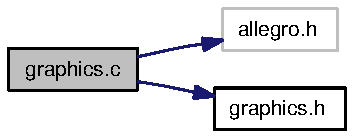
\includegraphics[width=103pt]{graphics_8c__incl}
\end{center}
\end{figure}
\subsection*{Funciones}
\begin{CompactItemize}
\item 
void \hyperlink{graphics_8c_c792bc74222685f93edc651253c59ed0_c792bc74222685f93edc651253c59ed0}{init\_\-graphics} ()
\item 
void \hyperlink{graphics_8c_e3919e2797a81eb7088a6b6f6b33bea7_e3919e2797a81eb7088a6b6f6b33bea7}{draw\_\-rect} (float minx, float miny, float maxx, float maxy, int r, int g, int b)
\item 
void \hyperlink{graphics_8c_a4f2f5f853228f62323d3c4d81c34a13_a4f2f5f853228f62323d3c4d81c34a13}{draw\_\-line} (float x1, float y1, float x2, float y2)
\item 
void \hyperlink{graphics_8c_9a7e11a2a03b0db3ab57985098c3f8fe_9a7e11a2a03b0db3ab57985098c3f8fe}{getscreen} ()
\item 
void \hyperlink{graphics_8c_7a2327678651d3939af5eec9503333e8_7a2327678651d3939af5eec9503333e8}{relscreen} ()
\item 
void \hyperlink{graphics_8c_ff4bc17c602603d120756f52e18ebb96_ff4bc17c602603d120756f52e18ebb96}{clearscreen} ()
\end{CompactItemize}


\subsection{Documentaci\'{o}n de las funciones}
\hypertarget{graphics_8c_ff4bc17c602603d120756f52e18ebb96_ff4bc17c602603d120756f52e18ebb96}{
\index{graphics.c@{graphics.c}!clearscreen@{clearscreen}}
\index{clearscreen@{clearscreen}!graphics.c@{graphics.c}}
\subsubsection[clearscreen]{\setlength{\rightskip}{0pt plus 5cm}void clearscreen ()}}
\label{graphics_8c_ff4bc17c602603d120756f52e18ebb96_ff4bc17c602603d120756f52e18ebb96}




Definici\'{o}n en la l\'{\i}nea 52 del archivo graphics.c.

\begin{Code}\begin{verbatim}52                   {
53 #if graphics
54 clear_bitmap(screen);
55 #endif
56 }
\end{verbatim}\end{Code}




Here is the caller graph for this function:\begin{figure}[H]
\begin{center}
\leavevmode
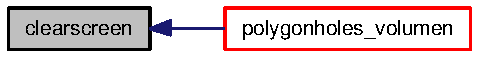
\includegraphics[width=133pt]{graphics_8c_ff4bc17c602603d120756f52e18ebb96_ff4bc17c602603d120756f52e18ebb96_icgraph}
\end{center}
\end{figure}
\hypertarget{graphics_8c_a4f2f5f853228f62323d3c4d81c34a13_a4f2f5f853228f62323d3c4d81c34a13}{
\index{graphics.c@{graphics.c}!draw_line@{draw\_\-line}}
\index{draw_line@{draw\_\-line}!graphics.c@{graphics.c}}
\subsubsection[draw\_\-line]{\setlength{\rightskip}{0pt plus 5cm}void draw\_\-line (float {\em x1}, float {\em y1}, float {\em x2}, float {\em y2})}}
\label{graphics_8c_a4f2f5f853228f62323d3c4d81c34a13_a4f2f5f853228f62323d3c4d81c34a13}




Definici\'{o}n en la l\'{\i}nea 34 del archivo graphics.c.

\begin{Code}\begin{verbatim}34                                                       {
35 #if graphics
36     line(screen,(int)x1,(int)y1,(int)x2,(int)y2,makecol(255,0,0));
37 #endif
38 }
\end{verbatim}\end{Code}




Here is the caller graph for this function:\begin{figure}[H]
\begin{center}
\leavevmode
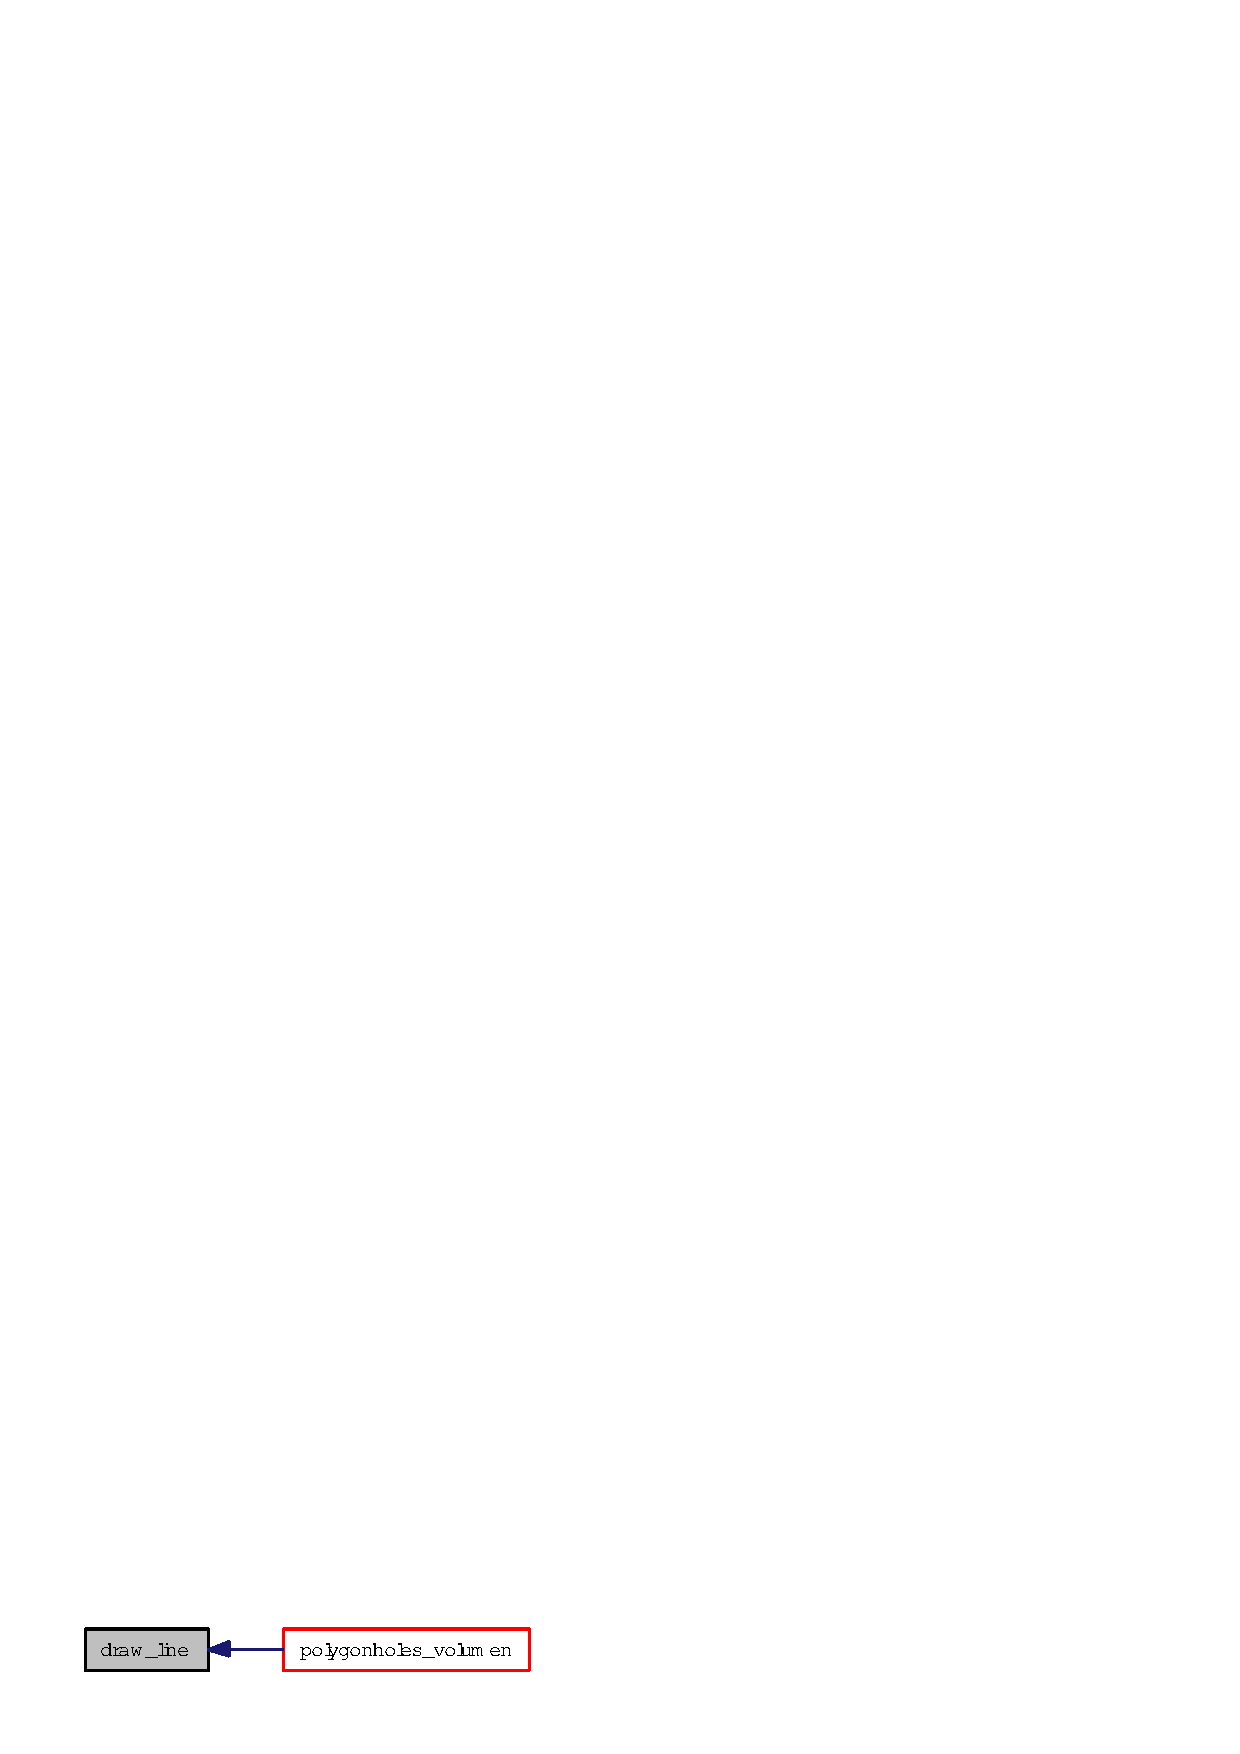
\includegraphics[width=129pt]{graphics_8c_a4f2f5f853228f62323d3c4d81c34a13_a4f2f5f853228f62323d3c4d81c34a13_icgraph}
\end{center}
\end{figure}
\hypertarget{graphics_8c_e3919e2797a81eb7088a6b6f6b33bea7_e3919e2797a81eb7088a6b6f6b33bea7}{
\index{graphics.c@{graphics.c}!draw_rect@{draw\_\-rect}}
\index{draw_rect@{draw\_\-rect}!graphics.c@{graphics.c}}
\subsubsection[draw\_\-rect]{\setlength{\rightskip}{0pt plus 5cm}void draw\_\-rect (float {\em minx}, float {\em miny}, float {\em maxx}, float {\em maxy}, int {\em r}, int {\em g}, int {\em b})}}
\label{graphics_8c_e3919e2797a81eb7088a6b6f6b33bea7_e3919e2797a81eb7088a6b6f6b33bea7}




Definici\'{o}n en la l\'{\i}nea 28 del archivo graphics.c.

\begin{Code}\begin{verbatim}28                                                                                   {
29 #if graphics
30 //    rect(screen, (int)minx, (int)miny, (int) maxx, (int) maxy, makecol(r,g,b));
31 #endif
32 }
\end{verbatim}\end{Code}




Here is the caller graph for this function:\begin{figure}[H]
\begin{center}
\leavevmode
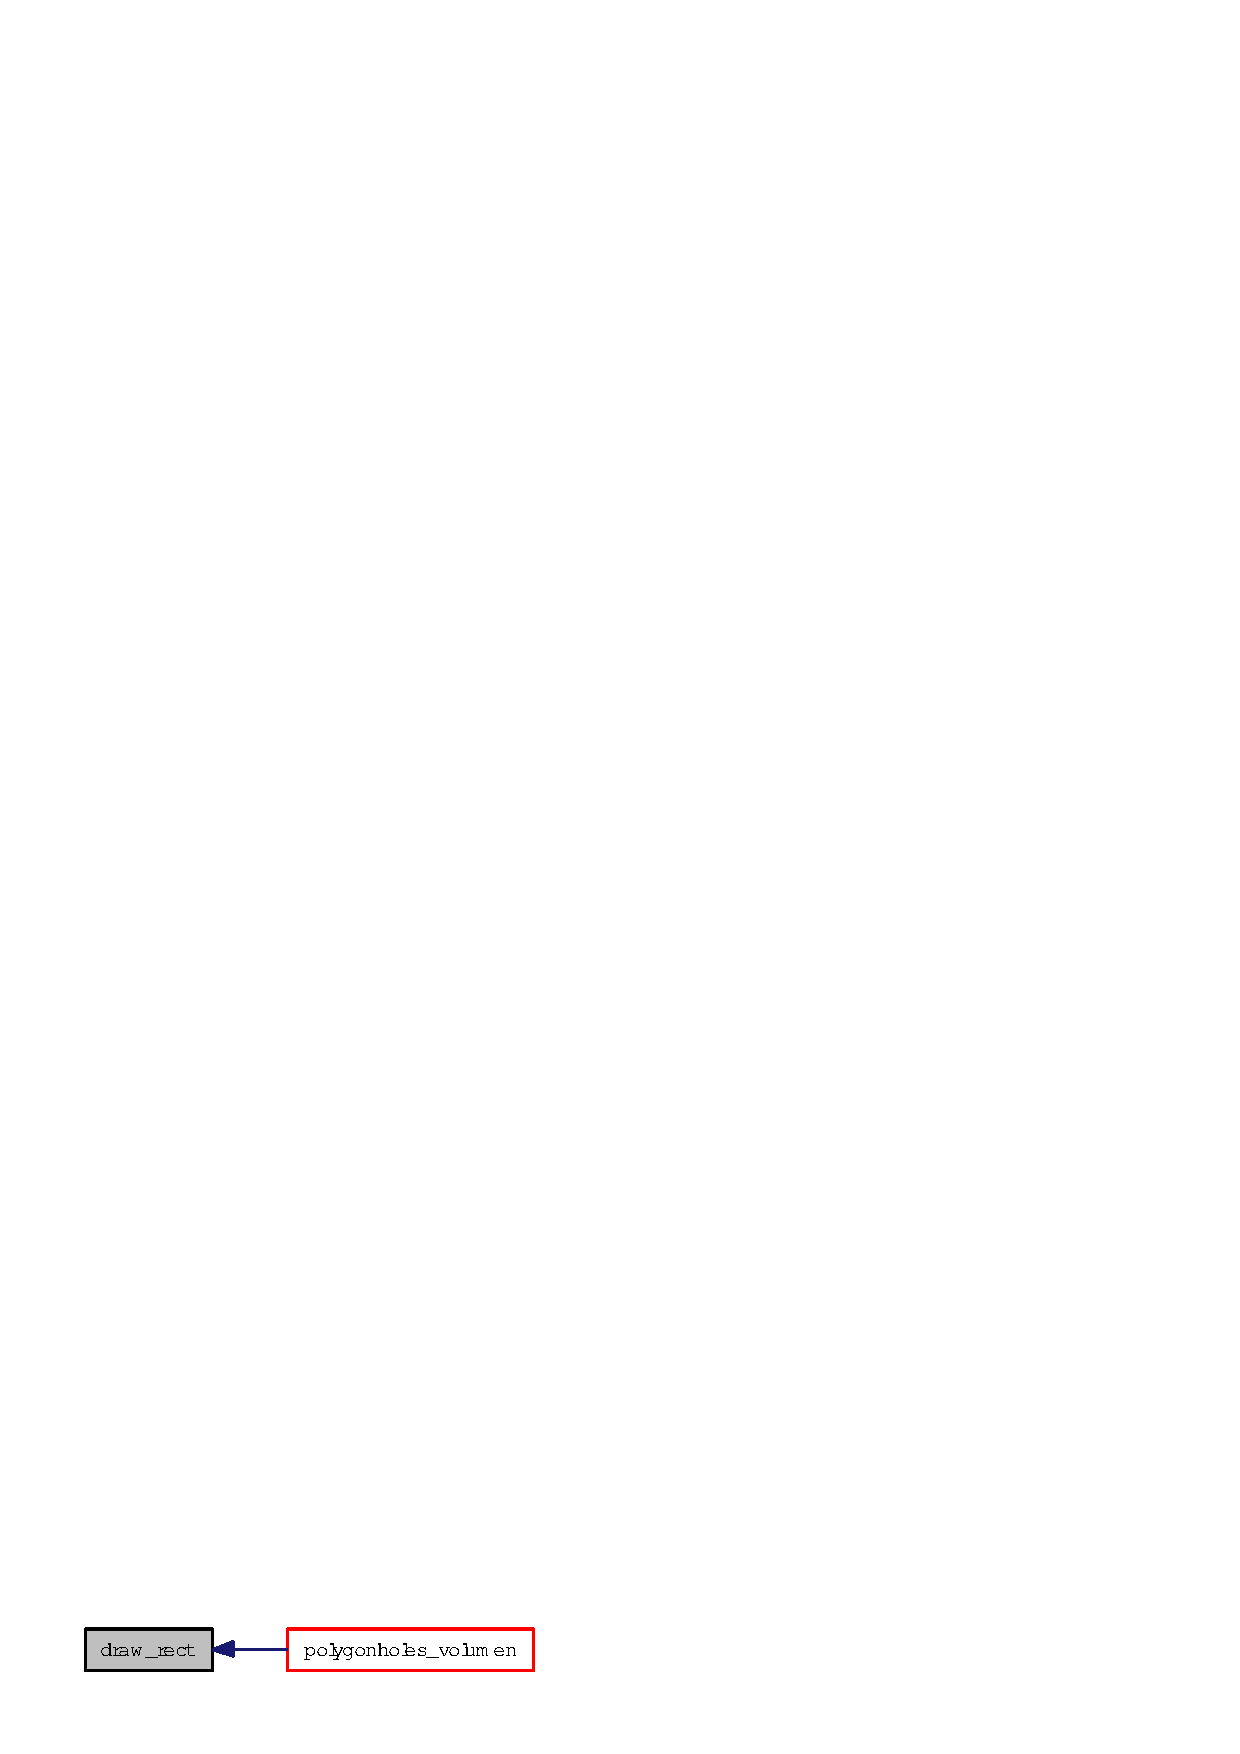
\includegraphics[width=130pt]{graphics_8c_e3919e2797a81eb7088a6b6f6b33bea7_e3919e2797a81eb7088a6b6f6b33bea7_icgraph}
\end{center}
\end{figure}
\hypertarget{graphics_8c_9a7e11a2a03b0db3ab57985098c3f8fe_9a7e11a2a03b0db3ab57985098c3f8fe}{
\index{graphics.c@{graphics.c}!getscreen@{getscreen}}
\index{getscreen@{getscreen}!graphics.c@{graphics.c}}
\subsubsection[getscreen]{\setlength{\rightskip}{0pt plus 5cm}void getscreen ()}}
\label{graphics_8c_9a7e11a2a03b0db3ab57985098c3f8fe_9a7e11a2a03b0db3ab57985098c3f8fe}




Definici\'{o}n en la l\'{\i}nea 40 del archivo graphics.c.

\begin{Code}\begin{verbatim}40                 {
41 #if graphics
42      acquire_screen();
43 #endif
44 }
\end{verbatim}\end{Code}




Here is the caller graph for this function:\begin{figure}[H]
\begin{center}
\leavevmode
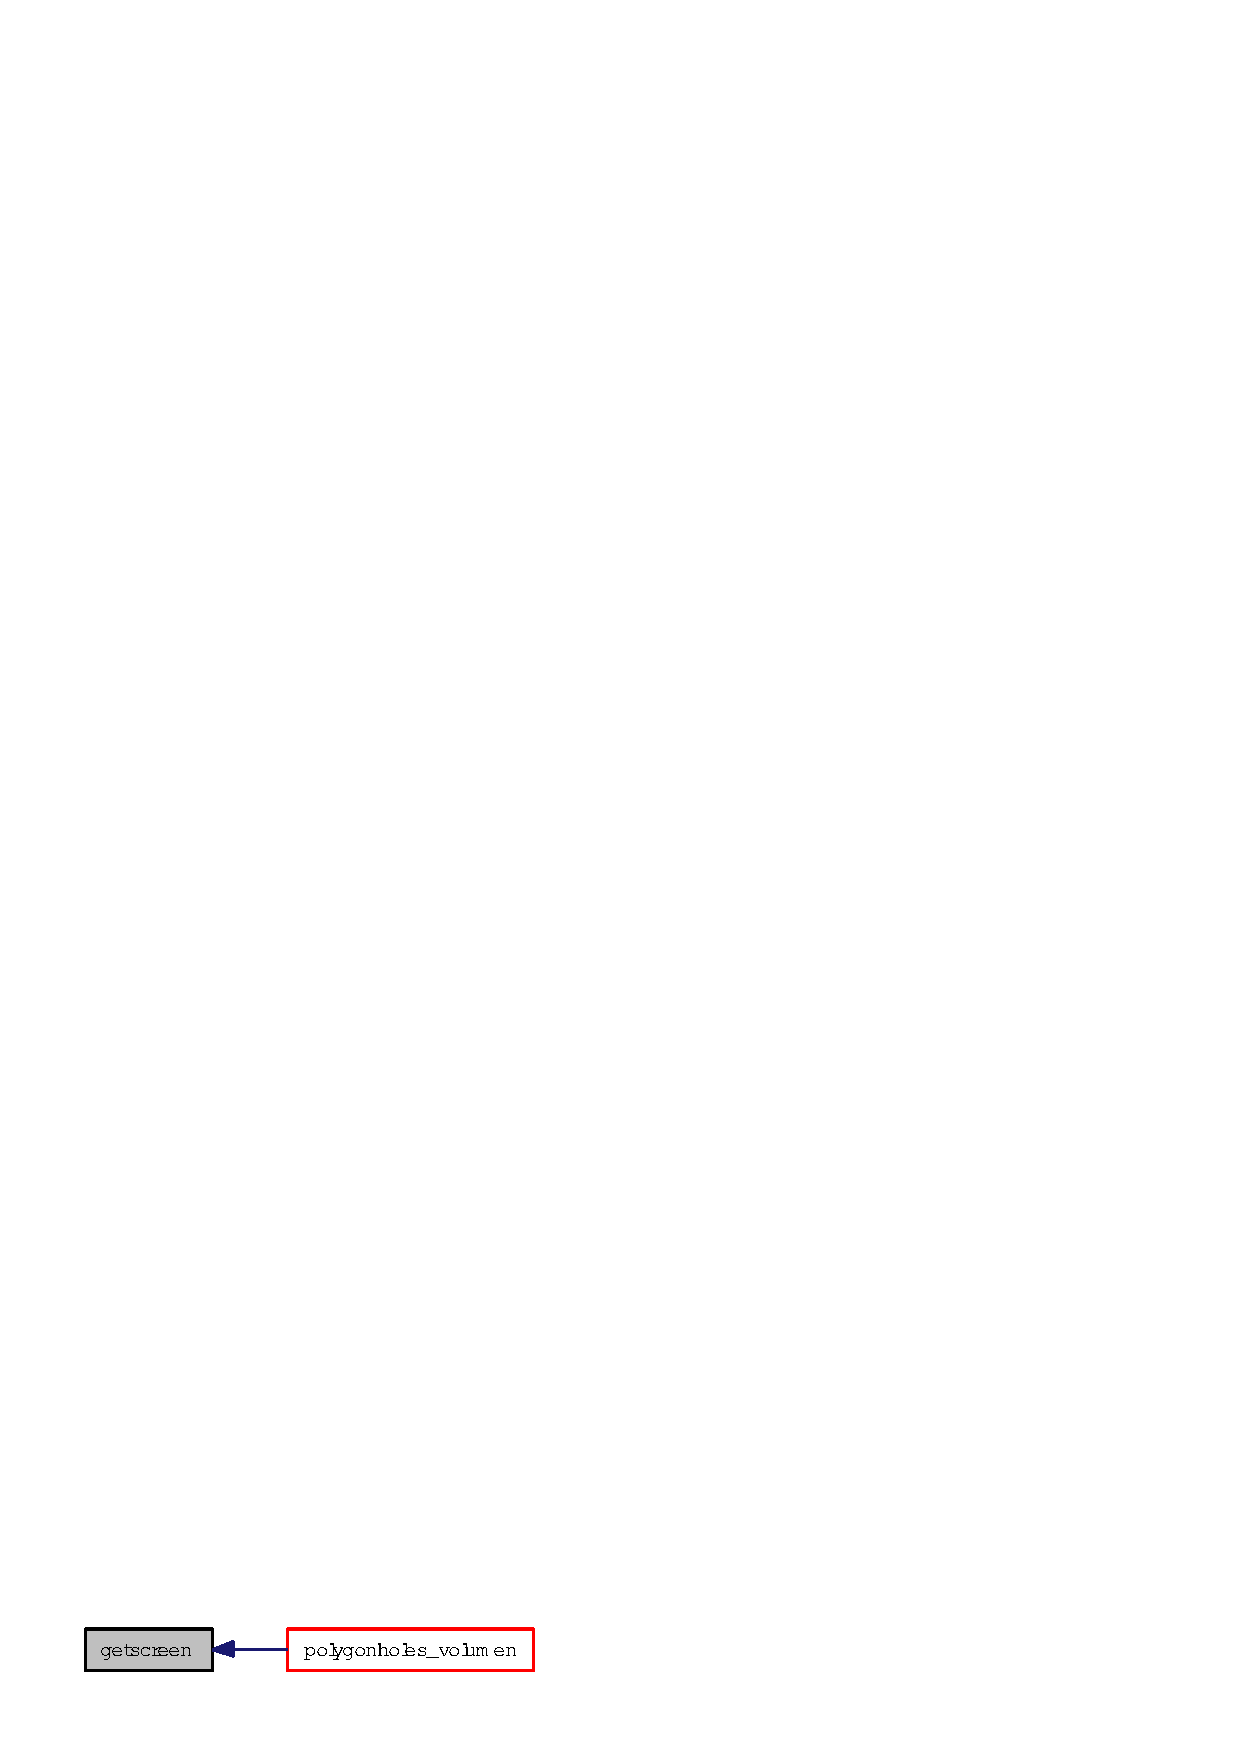
\includegraphics[width=130pt]{graphics_8c_9a7e11a2a03b0db3ab57985098c3f8fe_9a7e11a2a03b0db3ab57985098c3f8fe_icgraph}
\end{center}
\end{figure}
\hypertarget{graphics_8c_c792bc74222685f93edc651253c59ed0_c792bc74222685f93edc651253c59ed0}{
\index{graphics.c@{graphics.c}!init_graphics@{init\_\-graphics}}
\index{init_graphics@{init\_\-graphics}!graphics.c@{graphics.c}}
\subsubsection[init\_\-graphics]{\setlength{\rightskip}{0pt plus 5cm}void init\_\-graphics ()}}
\label{graphics_8c_c792bc74222685f93edc651253c59ed0_c792bc74222685f93edc651253c59ed0}




Definici\'{o}n en la l\'{\i}nea 6 del archivo graphics.c.

\begin{Code}\begin{verbatim}7 {
8 #if graphics
9     int depth, res;
10     allegro_init();
11     depth = desktop_color_depth();
12     if (depth == 0)
13         depth = 32;
14     set_color_depth(depth);
15     res = set_gfx_mode(GFX_AUTODETECT_WINDOWED, 640, 480, 0, 0);
16     if (res != 0)
17     {
18         allegro_message(allegro_error);
19         exit(-1);
20     }
21 
22     install_timer();
23     //install_keyboard();
24     //install_mouse();
25 #endif
26 }
\end{verbatim}\end{Code}




Here is the caller graph for this function:\begin{figure}[H]
\begin{center}
\leavevmode
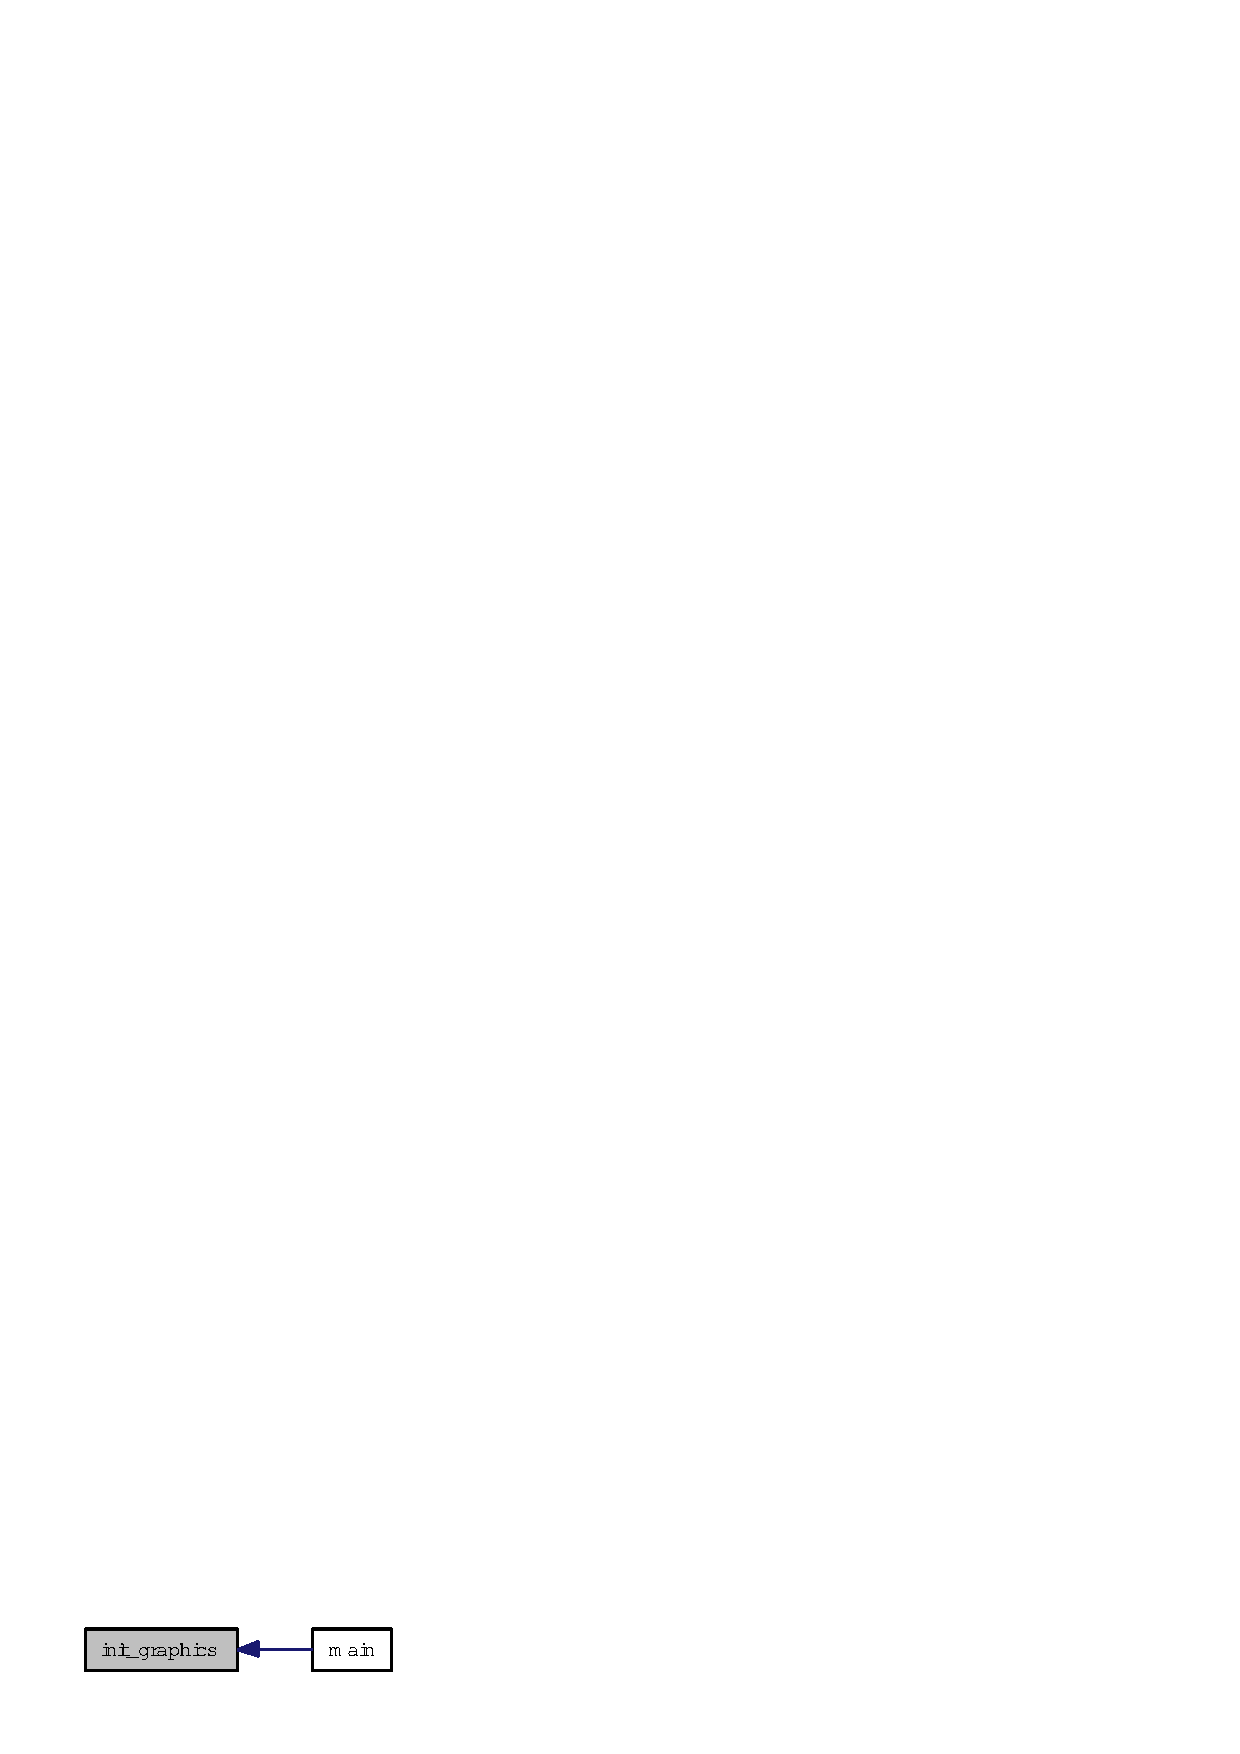
\includegraphics[width=96pt]{graphics_8c_c792bc74222685f93edc651253c59ed0_c792bc74222685f93edc651253c59ed0_icgraph}
\end{center}
\end{figure}
\hypertarget{graphics_8c_7a2327678651d3939af5eec9503333e8_7a2327678651d3939af5eec9503333e8}{
\index{graphics.c@{graphics.c}!relscreen@{relscreen}}
\index{relscreen@{relscreen}!graphics.c@{graphics.c}}
\subsubsection[relscreen]{\setlength{\rightskip}{0pt plus 5cm}void relscreen ()}}
\label{graphics_8c_7a2327678651d3939af5eec9503333e8_7a2327678651d3939af5eec9503333e8}




Definici\'{o}n en la l\'{\i}nea 46 del archivo graphics.c.

\begin{Code}\begin{verbatim}46                 {
47 #if graphics
48     release_screen();
49 #endif
50 }
\end{verbatim}\end{Code}




Here is the caller graph for this function:\begin{figure}[H]
\begin{center}
\leavevmode
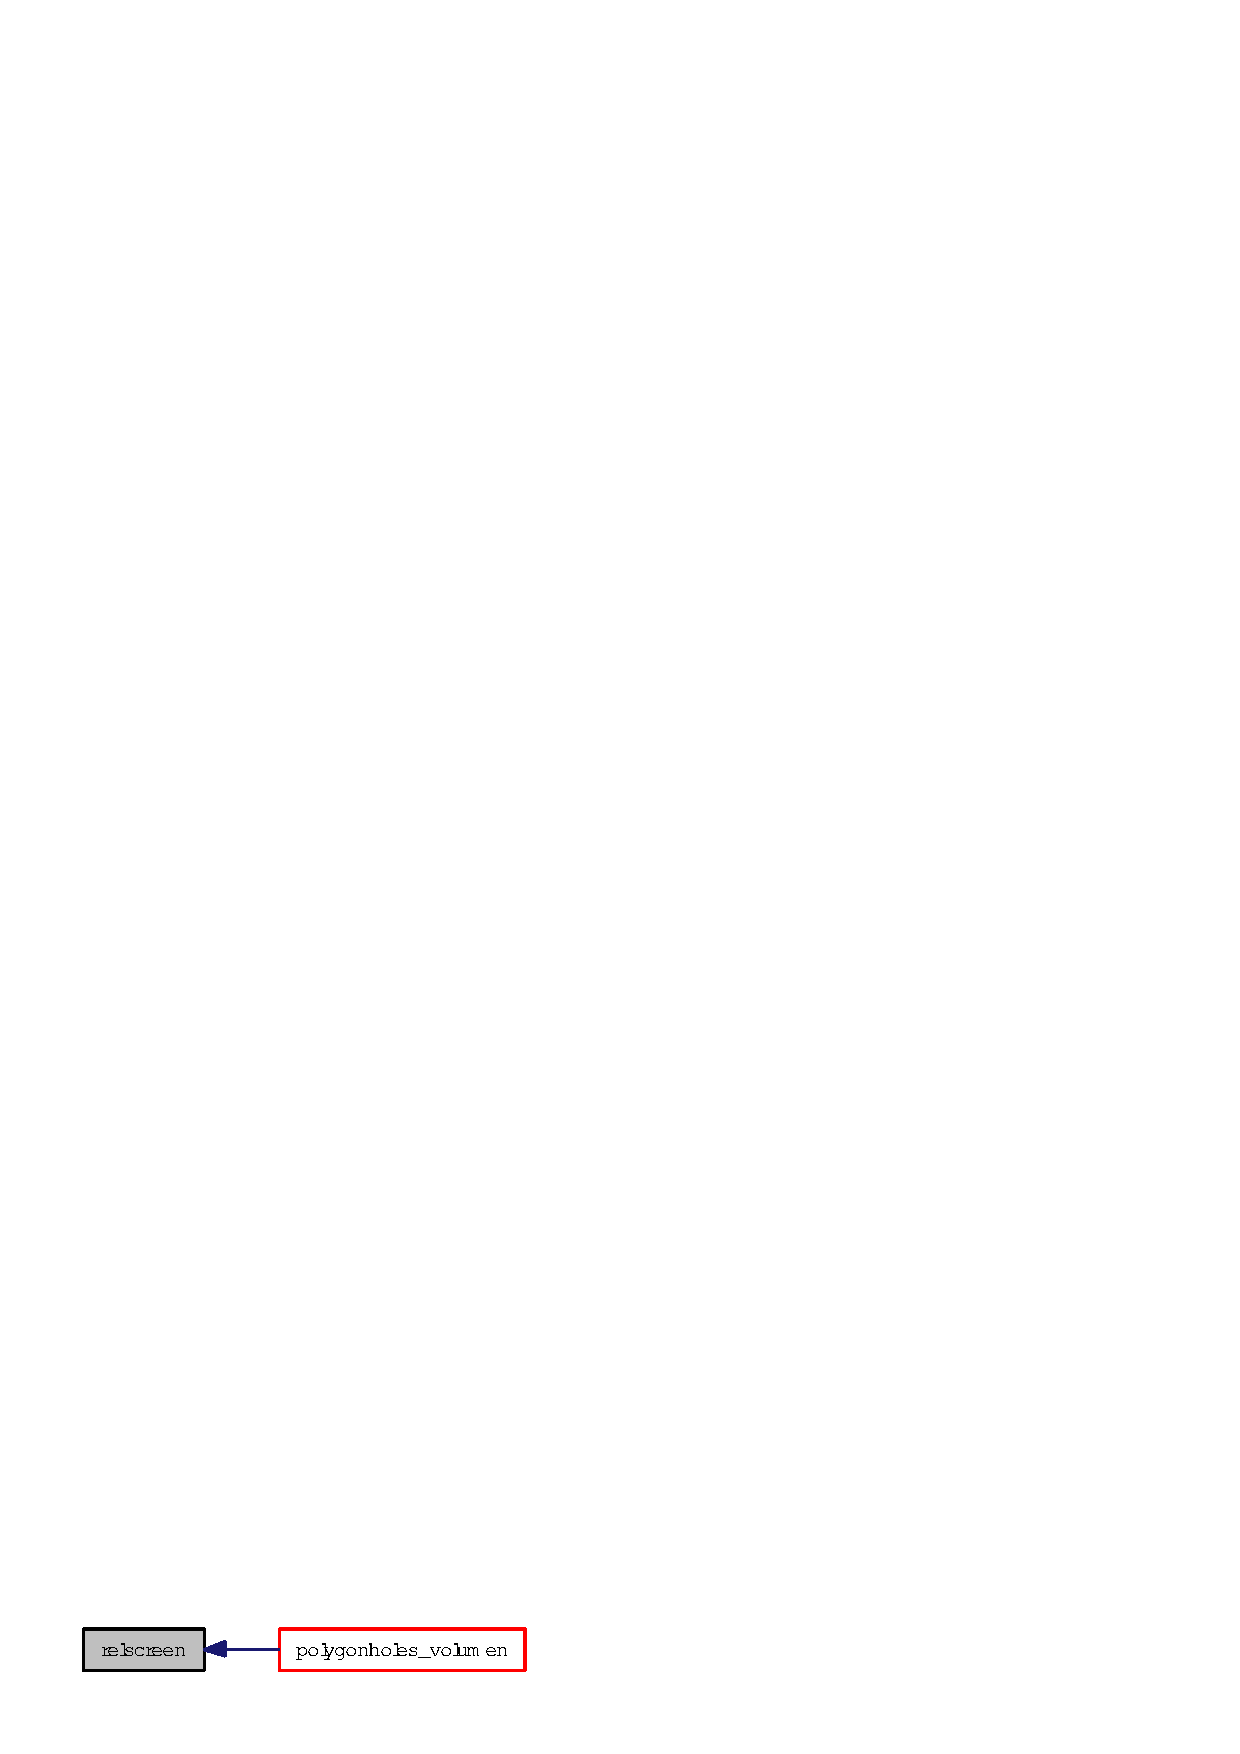
\includegraphics[width=128pt]{graphics_8c_7a2327678651d3939af5eec9503333e8_7a2327678651d3939af5eec9503333e8_icgraph}
\end{center}
\end{figure}
